\documentclass[10pt]{article}
\usepackage{../setup}
\vspace{-8ex}
\date{}

\graphicspath{ {./figs/} }

\begin{document}

\title{\textbf{\Large{\textsc{ECE410:} Linear Control Systems}} \\ \Large{Lab 3 Report: State Feedback Stabilization of a Cart-Pendulum Robot} \\ \textbf{\small{PRA102}}\vspace{-0.3cm}}
\author{Pranshu Malik, Varun Sampat \\ \footnotesize{1004138916}, \footnotesize{1003859602}\vspace{-3cm}}

\maketitle

\section{Inverted Cart-Pendulum Model}
In this lab, we consider a pendulum-cart system, similar to the one seen in lab 1, with the exception that the pendulum inverted; meaning the pendulum is linearized in its upright position. This lab also considers more system parameters such as the mass of the base ($M$). The control input, $u$, is defined as the force imparted at the point of pivot, being the cart base, which is free to move along a friction-less rod. We consider the state of the system to be $\vec{x} = \rcvec{x_1 & x_2 & x_3 & x_4}^\intercal = \rcvec{y & \dot{y} & \theta & \dot{\theta}}^\intercal$, where $\theta$ is the angle subtended by the pendulum rod against the vertically downwards axis and $y$ is the position of the cart on the horizontal axis. 

The pendulum has a mass $m$, of length $l$, and is subject to gravity, $g$. The system, as a whole, can be in \texttt{figure \ref{fig:inverted_pend}}

\begin{figure}[!h]
\centering
% \invertedpendcart
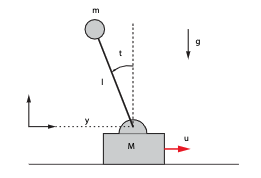
\includegraphics[0.8\linewidth]{lab3/inverted_cart_pend.png}
\caption{Invereted Cart-Pendulum system}
\label{fig:inverted_pend}
\end{figure}

The system is also subject to the following non-linear dynamics:
\begin{equation}
    \dot{y} = \frac{-l\,m\,\sin\left(\theta\right)\,{\dot{\theta}}^2+u+g\,m\,\cos\left(\theta\right)\,\sin\left(\theta\right)}{m\,{\sin\left(\theta\right)}^2+M}
\end{equation}

\begin{equation}
    \dot{\theta} = \frac{-l\,m\,\cos\left(\theta\right)\,\sin\left(\theta\right)\,{\dot{\theta}}^2+u\,\cos\left(\theta\right)+g\,\sin\left(\theta\right)\,\left(M+m\right)}{l\,\left(m\,{\sin\left(\theta\right)}^2+M\right)}
\end{equation}


\section{Analysing the cart pendulum model}
\subsection{Symbolic Representation of the linear system}

\begin{equation*}
    A = \left(\begin{array}{cccc} 0 & 1 & 0 & 0\\ 0 & 0 & \xi & -\frac{2\,l\,m\,x_{4}\,\sin\left(x_{3}\right)}{m\,{\sin\left(x_{3}\right)}^2+M}\\ 0 & 0 & 0 & 1\\ 0 & 0 & \mu & -\frac{2\,m\,x_{4}\,\cos\left(x_{3}\right)\,\sin\left(x_{3}\right)}{m\,{\sin\left(x_{3}\right)}^2+M} \end{array}\right)
\end{equation*}

where 
\begin{equation*}
    \xi = -\frac{m\,\left(l\,{x_{4}}^2\,\cos\left(x_{3}\right)-2\,g\,{\cos\left(x_{3}\right)}^2+g\right)}{-m\,{\cos\left(x_{3}\right)}^2+M+m}-\frac{2\,m\,\cos\left(x_{3}\right)\,\sin\left(x_{3}\right)\,\left(-l\,m\,\sin\left(x_{3}\right)\,{x_{4}}^2+u+g\,m\,\cos\left(x_{3}\right)\,\sin\left(x_{3}\right)\right)}{{\left(m\,{\sin\left(x_{3}\right)}^2+M\right)}^2}
\end{equation*}
and
\begin{multline*}
    \mu = -\frac{l\,m\,{x_{4}}^2\,{\cos\left(x_{3}\right)}^2-l\,m\,{x_{4}}^2\,{\sin\left(x_{3}\right)}^2-g\,\left(M+m\right)\,\cos\left(x_{3}\right)+u\,\sin\left(x_{3}\right)}{l\,\left(m\,{\sin\left(x_{3}\right)}^2+M\right)} \\ -\frac{2\,m\,\cos\left(x_{3}\right)\,\sin\left(x_{3}\right)\,\left(-l\,m\,\cos\left(x_{3}\right)\,\sin\left(x_{3}\right)\,{x_{4}}^2+u\,\cos\left(x_{3}\right)+g\,\sin\left(x_{3}\right)\,\left(M+m\right)\right)}{l\,{\left(m\,{\sin\left(x_{3}\right)}^2+M\right)}^2}
\end{multline*}

\begin{equation*}
    B_\text{} = 
    \left(\begin{array}{c} 0\\ \frac{1}{m\,{\sin\left(x_{3}\right)}^2+M}\\ 0\\ \frac{\cos\left(x_{3}\right)}{l\,\left(m\,{\sin\left(x_{3}\right)}^2+M\right)} \end{array}\right)
\end{equation*}

\subsection{Numerical Representation of the linear system}
The system parameters used in this lab are listed in the \texttt{table \ref{tab:sys_param}}:
\begin{table}[hbt!]
    \centering
    \begin{tabular}{c|c}
    \textbf{Parameters} & \textbf{Values} \\
    \hline
         $M$ & $1.0731$ kg \\
         $m$ & $0.2300$ kg \\
         $l$ & $0.3302$ m \\
         $g$ & $9.8$ m/$\text{s}^2$
    \end{tabular}
    \caption{Pendulum Parameters}
    \label{tab:sys_param}
\end{table}

Note that the system was linearized at the upright equilibrium point $\vec{x} = (0, 0, 0, 0)$

The numerical values for $A$ and $B$ can be computed using the equilibrium point, the symbolic representation of the linearized system, and the parameters defined above:

\begin{equation*}
    A = \left(\begin{array}{cccc} 0 & 1 & 0 & 0\\ 0 & 0 & \frac{g\,m}{M} & 0\\ 0 & 0 & 0 & 1\\ 0 & 0 & \frac{g\,\left(M+m\right)}{M\,l} & 0 \end{array}\right) = \left(\begin{array}{cccc} 0 & 1 & 0 & 0\\ 0 & 0 & 2.1005 & 0\\ 0 & 0 & 0 & 1\\ 0 & 0 & 36.0401 & 0 \end{array}\right)
\end{equation*}

\begin{equation*}
    B = \left(\begin{array}{c} 0\\ \frac{1}{M}\\ 0\\ \frac{1}{M\,l} \end{array}\right) = \left(\begin{array}{c} 0\\ 0.9319\\ 0\\ 2.8222 \end{array}\right)
\end{equation*}

\section{Controllability and Pole Assignment}

\subsection{Gain vectors $K_1$, $K_2$}
$K_1$ is defined as the gain vector such that the poles of the closed-loop system are located at p $ =\{-1, -2, -3, -4\}$. $K_1$ and $K_2$ were computed using the \texttt{MATLAB} command, \texttt{place(A, B, p)}:

\begin{equation*}
    K_1 = \rcvec{0.8677 & 1.8078 & -25.4584 & -4.1403}
\end{equation*}

\begin{equation*}
    K_2 = \rcvec{4.3387  &  8.1713 & -60.6206 & -11.9109}
\end{equation*}

\subsection{Plots}
Note: all these plots correspond to the initial condition $\vec{x_0} = \rcvec{ -0.5 & 0 & -\pi/4 & 0}^T$. Physically speaking, this corresponds to the cart $0.5$m to the left of the equilibrium and the pendulum is rotated 45$\deg$ clockwise.  
\subsection{Differences in Transient Response}
\subsection{}

\section{LQR}
Optimality does not ensure performance always.

\subsection{Impact of changing $q_1$}
For this subsection, $q_2$ and $R$ were fixed at $q_2$ = 5 and $R$ = 0.5. Two sets of gains were computed for $q_1$ = 0.1 and $q_1$ = 0.005.

\subsection{Impact of changing $q_2$}
For this subsection, $q_1$ and $R$ were fixed at $q_1$ = 0.05 and $R$ = 0.5. Two sets of gains were computed for $q_2$ = 1 and $q_2$ = 2000.

\subsection{Impact of changing $R$}
For this subsection, $q_1$ and $q_2$ were fixed at $q_1$ = 0.05 and $q_2$ = 5. Two sets of gains were computed for $R$ = 0.005 and $R$ = 10.

\section{Discussion on the impact of LQR on the nonlinear system}

\end{document}